%% \documentclass[twocolumn]{article}
\documentclass[pre,twocolumn,twoside,byrevtex,superscriptaddress]{revtex4}

\usepackage{amsmath}
\usepackage{amssymb}
\usepackage{url}
\usepackage{graphicx}
\usepackage{listings,color}
\usepackage{setspace}

\lstset{language=matlab,
        basicstyle=\ttfamily\scriptsize\singlespacing,
        keywordstyle=\color{blue},
        stringstyle=\color{red},
        commentstyle=\color{green},
        morecomment=[l][\color{magenta}]{\#},
        frame=L,
        xleftmargin=\parindent,
        numbersep=5pt,
        breaklines=true,
        breakatwhitespace=false,
        escapeinside={\%*}{*)},
}

\setlength{\parindent}{0cm}

\setlength{\parskip}{1mm}

\begin{document}

%% \twocolumn[
%%   \begin{@twocolumnfalse} 

%%     \title{\vspace{-2cm}Homework 4: Counterprop}
%%     \author{Andy Reagan}

%%     \maketitle

%%   \end{@twocolumnfalse}
%% ]

\title{\vspace{-2cm}Homework 5: SOM}
\author{Andy Reagan}

\begin{abstract}
I code and discuss an implementation of Kohonen's original SOM.
\end{abstract}

\maketitle


\section{Introduction}

Originally proposed by Kohonen, the self organizing map describes a general class of unsupervised artificial nueral networks \cite{kohonen1990self}.

%% \begin{figure}[h]
%%  \centering
%%   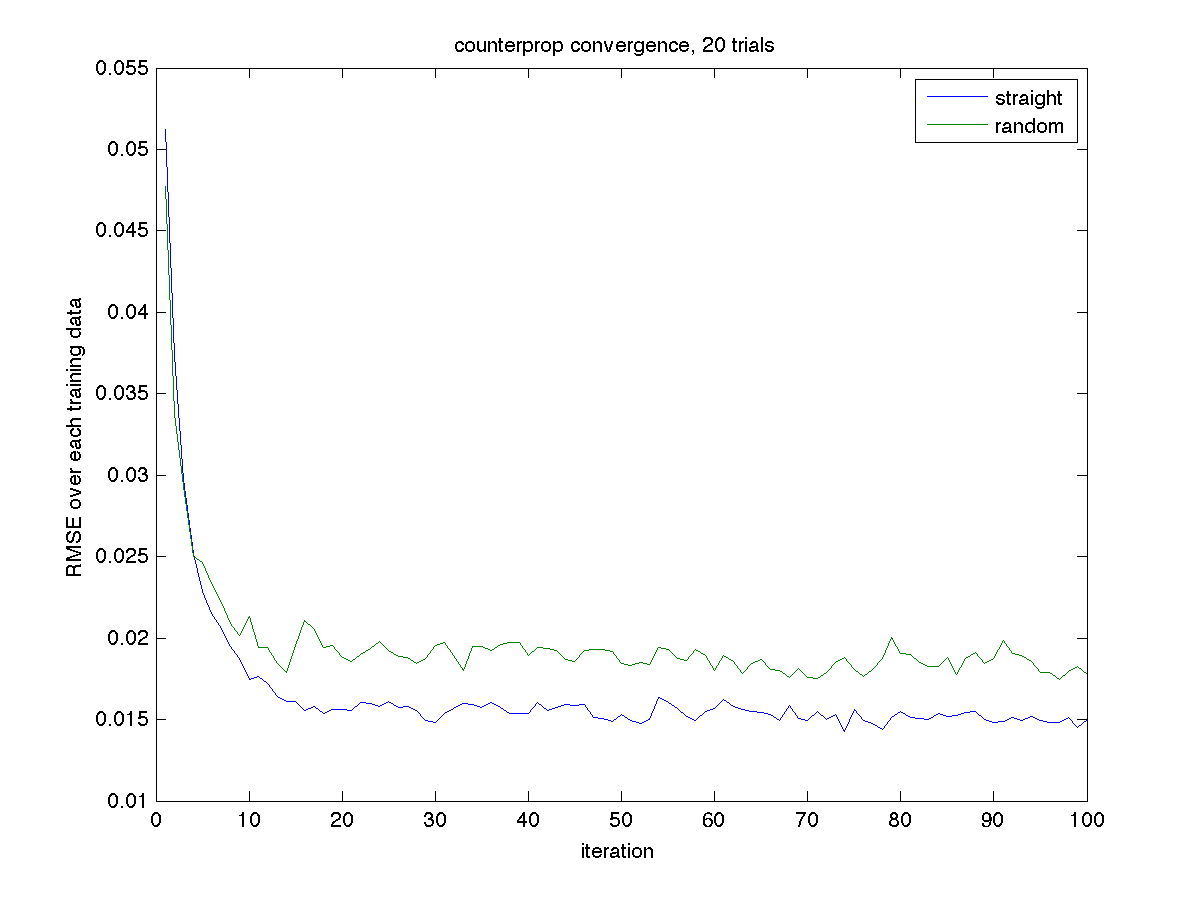
\includegraphics[width=0.48\textwidth]{115.png}
%%   \label{fig:5}
%%   \caption{Direct comparison over 100 trials of the convergence when presenting training data in a random or repeated order.}
%% \end{figure}



\clearpage
\pagebreak

\bibliographystyle{chicago}
\bibliography{writeup}

\clearpage
\pagebreak
\onecolumngrid

    \section*{Full code}

    \lstinputlisting{SOM_andy_driver.m}

    \lstinputlisting{train_SOM.m}

\clearpage
\pagebreak

    \section*{Extra figures}

    %% \begin{figure}
    %%   \centering
    %%   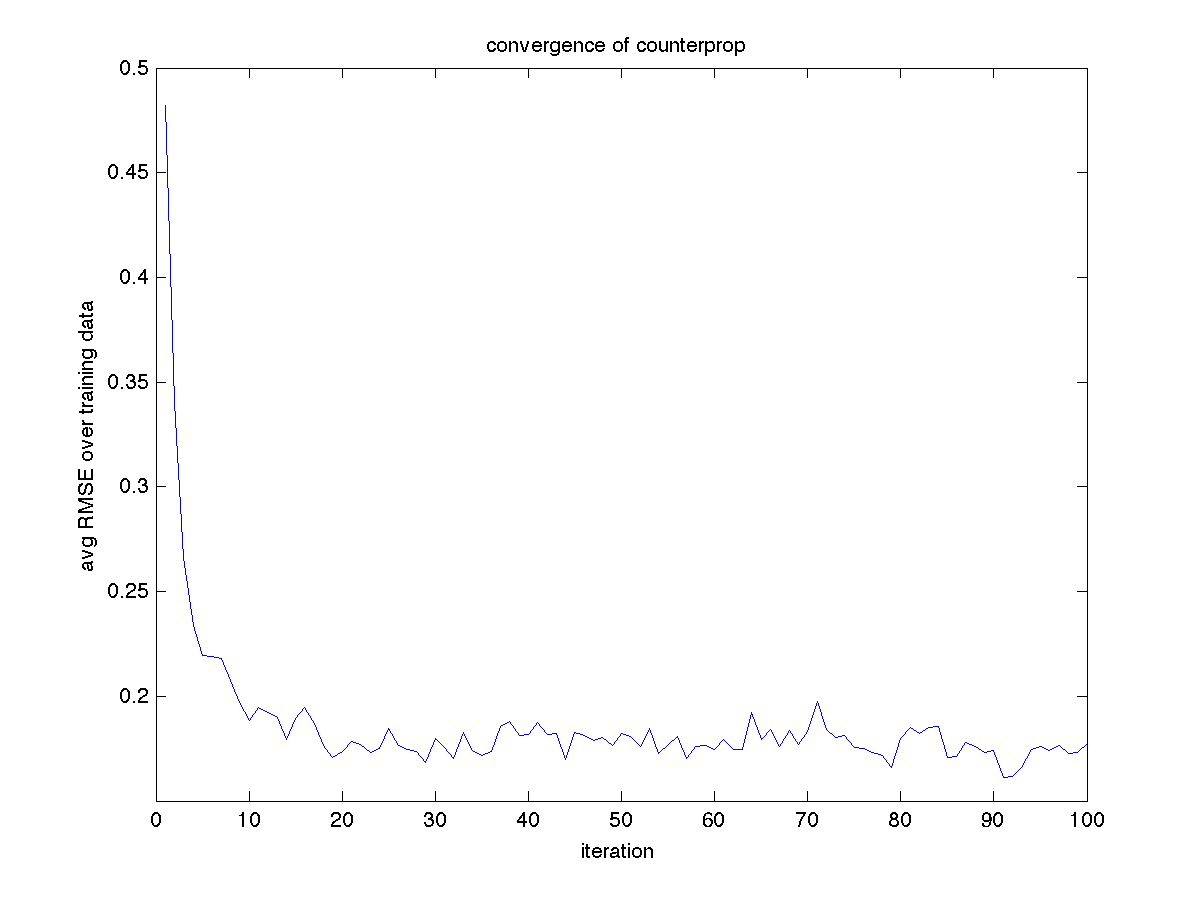
\includegraphics[width=0.68\textwidth]{111.png}
    %%   \label{fig:1}
    %%   \caption{Basic convergence test.}
    %% \end{figure}

\end{document}
